\section*{CHAPTER 3:  DESIGN AND IMPLEMENTATION}
\addcontentsline{toc}{section}{\numberline{}CHAPTER 3: DESIGN AND IMPLEMENTATION}
\setcounter{section}{3}
\setcounter{subsection}{0}
\setcounter{figure}{0}
\setcounter{table}{0}

\subsection{OFDM Modulation method and transceiver architechure}
Orthogonal Frequency Division Multiplexing (OFDM) modulation is based on the Frequency Division Multiplexing (FDM) technique, with the key distinction that the subcarrier waves are placed orthogonally to each other. With this orthogonality, their signal spectra overlap without affecting the demodulation process at the receiver. The signal spectrum of a system of subcarrier waves is illustrated in Figure \ref{Spectrum} \cite{b6}.

\begin{figure}[htbp]
    \centering
    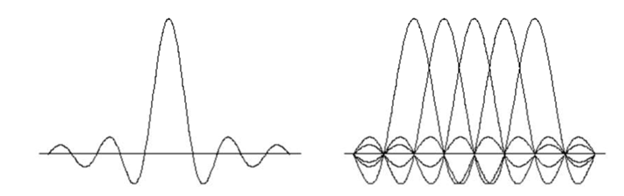
\includegraphics[width=\textwidth]{Figures/Spectrum.png}
    \caption{\bfseries\centering\fontsize{13pt}{0pt}\selectfont Spectrum of a single subcarrier (left) and 5 subcarriers (right)}
    \label{Spectrum}    
\end{figure}

As shown in Figure \ref{Spectrum}, the signal spectrum of each subcarrier channel has the form of $\frac{sin(x)}{x}$. The subcarriers are distributed evenly across the frequency range, ensuring that the peak points of one channel coincide with the null points of adjacent subcarrier channels. In the OFDM system, the signals, after passing through the digital modulator, undergo an Inverse Fast Fourier Transform (IFFT) to form OFDM symbols. The use of IFFT allows the OFDM modulator to simultaneously modulate multiple channels, a task that is challenging with FDM modulators.

\begin{figure}[htbp]
    \centering
    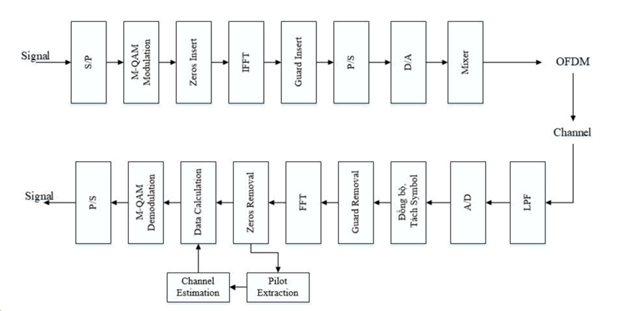
\includegraphics[width=\textwidth]{Figures/Block-diagram.png}
    \caption{\bfseries\centering\fontsize{13pt}{0pt}\selectfont Block diagram of the OFDM system}
    \label{Block diagram}    
\end{figure}

Principles of operation for each block:
\begin{itemize}
    \item S/P (Serial to Parallel): Converts serial data into parallel data, splitting high-speed bit streams into K lower-speed bit streams, where K is the number of subcarrier waves in the system.
    \item M-QAM Modulation: Utilizes QAM modulation to map pairs of bits into complex signals in the QAM signal constellation. The modulation level M is chosen based on different transmission systems.
    \item Zero Insertion: Inserts virtual subcarriers to ensure the DC component's average value is zero and creates a frequency guard band between information systems to avoid Intercarrier Interference (ICI).
    \item IFFT (Inverse Fast Fourier Transform): Performs a fast implementation of the Inverse Discrete Fourier Transform, transforming signals from the time domain to the frequency domain, creating orthogonal subcarrier waves.
    \begin{equation}
        x_n = \frac{1}{N} \sum_{k=0}^{N-1} X_k . e^\frac{j2\pi kn}{N}
    \end{equation}
    \item Guard Insertion: Inserts a guard interval to counteract Inter-Symbol Interference (ISI). ISI arises from the influence of multipath effects when symbols arriving later interfere with symbols arriving earlier. The guard interval length depends on the transmission channel and follows the principle of copying a portion of the signal sequence that needs to be transmitted and appending it to the beginning of the signal.
    \item P/S (Parallel to Serial): Converts parallel data back to serial, returning the signal stream to its original continuous form for transmission.
    \item Mixer: Combines the signal with carrier waves before sending it to the antenna. OFDM modulation uses two different Mixers for two streams of real and complex signals from the P/S block. These two signal streams are multiplied successively with carrier waves and then added at the Mixer's output.
    \item LPF (Low Pass Filter): Low-pass filter that brings the signal back to baseband.
    \item D/A, A/D: Converts signals from digital to analog and analog to digital for long-distance transmission. The signal after D/A conversion is an analog baseband signal with a bandwidth depending on the sampling frequency in the D/A converter. At the receiver, an A/D converter is used to obtain digital signals for decoding.
    \item Pilot Extraction, Channel Estimation: Based on pilot signals, the receiver estimates the transmission channel using estimation algorithms.
    \item 64-QAM Modulation/Demodulation: Maps binary sequences to complex signals characteristic of points in the QAM signal constellation. As illustrated in Figure \ref{Constellation}, each bit sequence corresponds to one point on the complex plane. Quadrature Amplitude Modulation (QAM) is a modulation technique that combines amplitude modulation and phase modulation. Compared to other modulation types, QAM signals can resist noise effectively because the receiver can differentiate based on both amplitude and phase. The symbol constellation of QAM signals has larger amplitude and phase differences than other modulation types with the same number of levels M, making it less susceptible to interference when symbols overlap.
\end{itemize}

\begin{figure}[htbp]
    \centering
    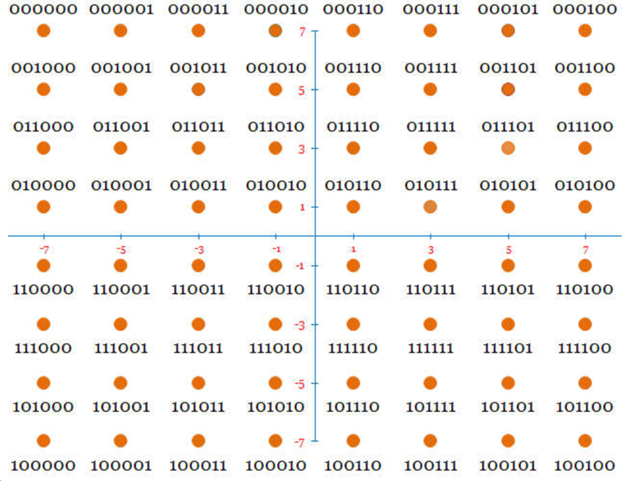
\includegraphics[width=\textwidth]{Figures/64-QAM-Constellation.png}
    \caption{\bfseries\centering\fontsize{13pt}{0pt}\selectfont 64-QAM Constellation}
    \label{Constellation}   
\end{figure}